% To submit: 2, 4
% Author: Abraham Murciano, Jonah Laurence

\begin{enumerate}
	\item[\textbf{1.}] % Abraham Murciano
		We are given the following differential equation.
		\[
			\dydx = 4xe^{2x}
		\]

		To find a solution, both sides can be integrated.
		\[
			y = 4 \int xe^{2x} dx
		\]

		Now integration by parts can be applied, with \(f(x) = x\) and \(g'(x) = e^{2x}\). This implies that \(f'(x) = 1\) and \(g(x) = \frac{1}{2}e^{2x}\). Therefore, by the rule of integration by parts,
		\[
			\int xe^{2x} dx = \frac{1}{2}xe^{2x} - \frac{1}{2} \int e^{2x} dx
		\]

		The next step is to calculate the integral of \(e^{2x}\). To do so, we will substitute \(u = 2x\).
		\[
			\int e^{2x} dx = \frac{1}{2} \int e^u du = \frac{1}{2} \cdot \frac{e^u}{\ln(e)} = \frac{1}{2} e^{2x} + c
		\]

		Therefore we have
		\begin{align*}
			y & = 4 \left(\frac{1}{2}xe^{2x} - \frac{1}{2} \left(\frac{1}{2} e^{2x}\right)\right) + c = 2xe^{2x} - e^{2x} + c \\
			  & = e^{2x} (2x-1) + c
		\end{align*}

		The graphs for \(y\) when \(c = -5, 0, 1, 4,\) and \(9\) can be seen in Figure \ref{q1b1}

		\begin{figure}[htb]
			\centering
			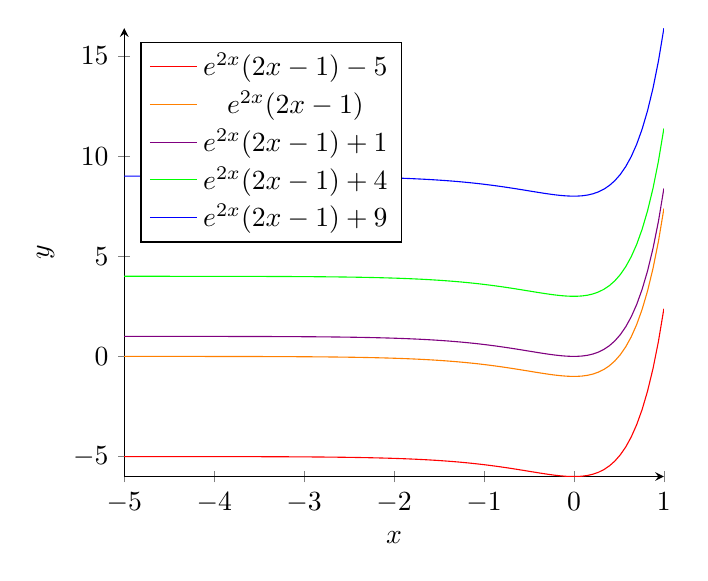
\begin{tikzpicture}
				\begin{axis}[
						legend pos=north west,
						axis lines = left,
						xlabel = \(x\),
						ylabel = \(y\),
					]

					\addplot [
						domain=-5:1,
						samples=100,
						color=red,
					]
					{e^(2*x) * (2*x-1) - 5};
					\addlegendentry{\(e^{2x} (2x-1) - 5\)}

					\addplot [
						domain=-5:1,
						samples=100,
						color=orange,
					]
					{e^(2*x) * (2*x-1)};
					\addlegendentry{\(e^{2x} (2x-1)\)}

					\addplot [
						domain=-5:1,
						samples=100,
						color=violet,
					]
					{(e^(2*x) * (2*x-1)) + 1};
					\addlegendentry{\(e^{2x} (2x-1) + 1\)}

					\addplot [
						domain=-5:1,
						samples=100,
						color=green,
					]
					{(e^(2*x) * (2*x-1)) + 4};
					\addlegendentry{\(e^{2x} (2x-1) + 4\)}

					\addplot [
						domain=-5:1,
						samples=100,
						color=blue,
					]
					{(e^(2*x) * (2*x-1)) + 9};
					\addlegendentry{\(e^{2x} (2x-1) + 9\)}

				\end{axis}
			\end{tikzpicture}
			\caption{\(y = e^{2x} (2x-1) + c\) when \(c = -5, 0, 1, 4,\) or \(9\)}
			\label{q1b1}
		\end{figure}

	\item[\textbf{2.}] % Jonah Laurence
		Given the following differential equation and values for the constant of integration
		\[y'(x) = x + 3, \qquad c= 0, 1, -6.\]

		We can integrate it to find \(y(x)\).
		\begin{gather*}
			y'(x) = x + 3\\
			\int y'(x) dx = \int (x + 3) dx\\
			y(x) = \frac{x^2}{2} + 3x + c
		\end{gather*}

		The graphs for \(y\) with the given values for \(c\) can be seen in Figure \ref{q1b2}

		\begin{figure}[htb]
			\centering
			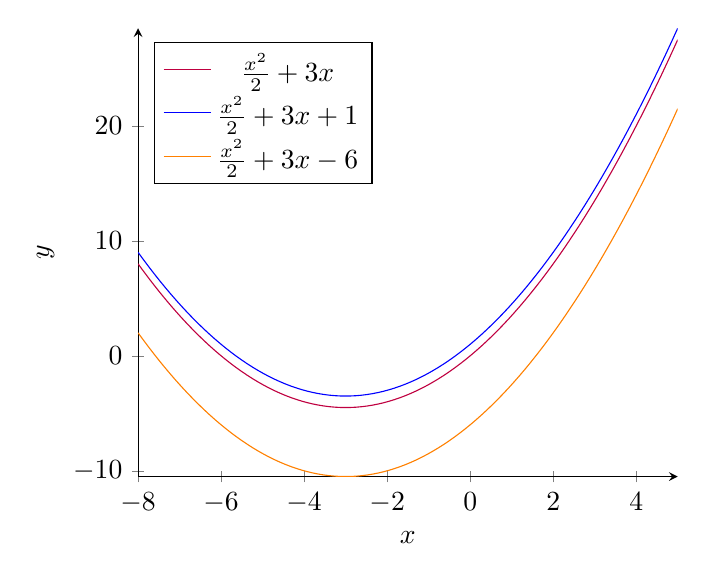
\begin{tikzpicture}
				\begin{axis}[
						legend pos=north west,
						axis lines = left,
						xlabel = \(x\),
						ylabel = {\(y\)},
					]
					\addplot [
						domain=-8:5,
						samples=100,
						color=purple,
					]
					{0.5 * x^2 + 3*x};
					\addlegendentry{\(\frac{x^2}{2} + 3x\)}
					\addplot [
						domain=-8:5,
						samples=100,
						color=blue,
					]
					{0.5 * x^2 + 3*x + 1};
					\addlegendentry{\(\frac{x^2}{2} + 3x + 1\)}
					\addplot [
						domain=-8:5,
						samples=100,
						color=orange,
					]
					{0.5 * x^2 + 3*x - 6};
					\addlegendentry{\(\frac{x^2}{2} + 3x - 6\)}
				\end{axis}
			\end{tikzpicture}
			\caption{\(y = e^{2x} (2x-1) + c\) when \(c = 0, 1,\) or \(-6\)}
			\label{q1b2}
		\end{figure}


	\item[\textbf{4.}] % Jonah Laurence
		We are given the following differential equation and certain pairs of values for \(x\) and \(y\).
		\[y'=\frac{2}{x} + 3,  \qquad y(1) = 0, y(1) = 1, y(-2) =-6\]

		We now integrate to find \(y\), and substitute the given values of \(x\) and \(y\) to find values for \(c\).
		\begin{gather*}
			y'=\frac{2}{x} + 3\\
			\int y'(x) dx = \int \left(\frac{2}{x} + 3\right) dx\\
			y(x) = 2 \ln x + 3x + c\\
			y(1) = 2 \ln (1) + 3(1) + c = 0\ \Rightarrow\ c = -3\\
			y(1) = 2 \ln (1) + 3(1) + c = 1\ \Rightarrow\ c = -2\\
			y(-2) = 2 \ln (-2) + 3(-2) + c = -6\ \Rightarrow\ c \text{ is undefined}
		\end{gather*}

		Once we have these, we can plot the graphs in Figure \ref{q1b4}.
		\begin{figure}[htb]
			\centering
			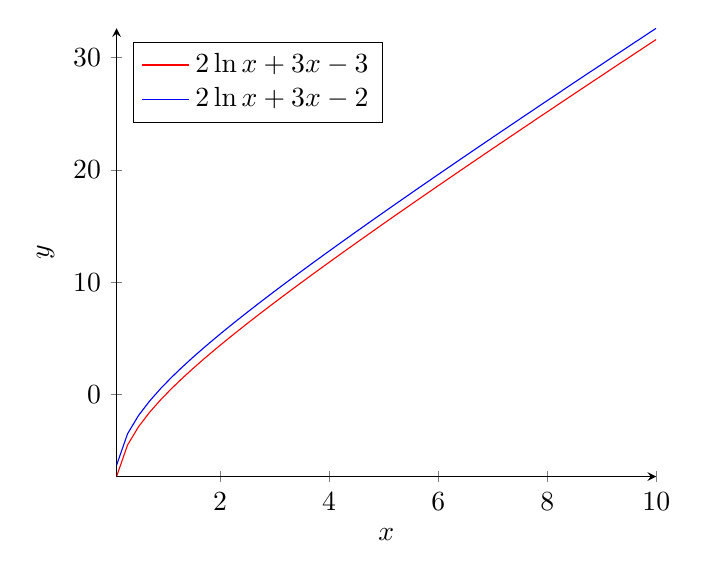
\begin{tikzpicture}
				\begin{axis}[
						legend pos=north west,
						axis lines = left,
						xlabel = \(x\),
						ylabel = \(y\),
					]

					\addplot [
						domain=-10:10,
						samples=100,
						color=red,
					]
					{2 * ln(x) + 3*x - 3};
					\addlegendentry{\(2 \ln x + 3x - 3\)}

					\addplot [
						domain=-10:10,
						samples=100,
						color=blue,
					]
					{2 * ln(x) + 3*x - 2};
					\addlegendentry{\(2 \ln x + 3x - 2\)}
				\end{axis}
			\end{tikzpicture}
			\caption{\(y = 2 \ln x + 3x + c\) when \(y(1) = 0, y(1) = 1, y(-2) = -6\)}
			\label{q1b4}
		\end{figure}
\end{enumerate}